% !TeX spellcheck = en_US
\documentclass[a4paper,twocolumn]{article}

\usepackage{fullpage}
\usepackage{fourier}
\usepackage{amsmath}
\usepackage{xcolor}
\usepackage{graphicx}
\usepackage{titlesec}
\usepackage{hyperref}
\usepackage{cleveref}
\usepackage{tabularx}

\titleformat{\subsection}[hang]{\large\bfseries}{\alph{subsection})\quad}{0pt}{}

\newcommand{\twodo}{\vspace{11pt}\textcolor{red}{\textbf{todo}}}
\newcommand{\subtask}[2]{\paragraph{#1)} \textit{#2} \newline}

\title{\textbf{Exercises for Image Processing 1}\\Problem Sheet 4}
\author{Axel Brand\\6145101 \and Nourhan Elfaramawy\\6517858 \and Sibel Toprak\\6712316}

\begin{document}
	\maketitle
	
	\section{Theoretical Problems}
	
	\subsection{Histogram and Noise}
	
	A histogram is a graphical representation that visualizes how many times certain values occur in some given data. The data could be for example an image, in which case the corresponding color histogram represents the color distribution as it would plot the number of pixels for each color value. Conventionally, the horizontal axis represents the values, while the vertical axis represents their number of occurrence.
	
	For an image showing white parcels on a black conveyor belt, the kind of histogram to expect is a gray-value histogram, which provides the discrete gray-value distribution within the image. More particularly, the distribution of the gray-values would be a bimodal one with two more or less clearly distinguishable peaks: For gray-values ranging from 0 (lightest) to 255 (darkest), there would be one peak within a range around 0 for the white parcels and another one within a range around 255 for the black conveyor belt.
	
	If the camera is affected by sensor noise, the histogram might change in that the peaks appear to be shifted or the strict bi-modality is lost: The gray-values are distributed more evenly such that the peaks cannot be clearly distinguished anymore. It is difficult to determine a threshold by which we can decide with high accuracy whether an area in the image corresponds to a part of the parcel or of the conveyor belt.
	
	\subsection{Projections}
		
	To separate the text in the image into lines, one could project the gray-values in an image in ``column profile''. This yields a column vector of row sums. The row sum will be way higher for rows showing parts of characters compared to the sum for rows in the image that are in-between text lines. By using an appropriate value as threshold, we can detect the text lines in the image.
	
	The extracted image strips showing a text line can then be processed further to separate the characters. To that end, a gray-value projection is performed on each image strip, but this time in ``row profile''. Using the resulting row vector of column sums, we can distinguish between columns that are involved in the rendering of the characters and those that show white spaces: The column sum for the former is way larger. Based on that, the characters can be extracted from these image strips using an appropriate threshold value.
	
	\subsection{Filters}
	
	\twodo{}
	% See \textbf{Image Processing, Analysis, and Machine Vision} by Milan Sonka, Vaclav Hlavac, Roger Boyle
	
	
	\subsection{Convolution}
	
	The convolution matrix  filter uses a first matrix which is the image to be treated in the spatial domain. The image is a bi-dimensional collection of pixels in rectangular coordinates, and the used kernel depends on the required task or the desired effect to be applied. We take into consideration a 3x3 Mask. The  filter studies successively every pixel of the image, and it multiplies the value of the initial pixel and values of the 8 surrounding pixels by the kernel corresponding value. Then, it sums the results, and the initial pixel is set to this summed result value.
	
	When applying the convolution of an image with itself, that will result in a convolution matrix that is equal in size to the original image B1, giving the weight of every pixel the value 1, so the value of every single pixel depends on the values of the pixels of the entire image, which will result in a more blurred and fuzzy optical effect in the image see B2.
	
	\begin{figure*} [t]
		\centering
		\begin{tabular}{c c}
			\includegraphics[width=0.8\columnwidth]{figures/B1.png}
			&
			
\includegraphics[width=0.8\columnwidth]{figures/B2.png}\\
			B1 & B2\\
			& \\
			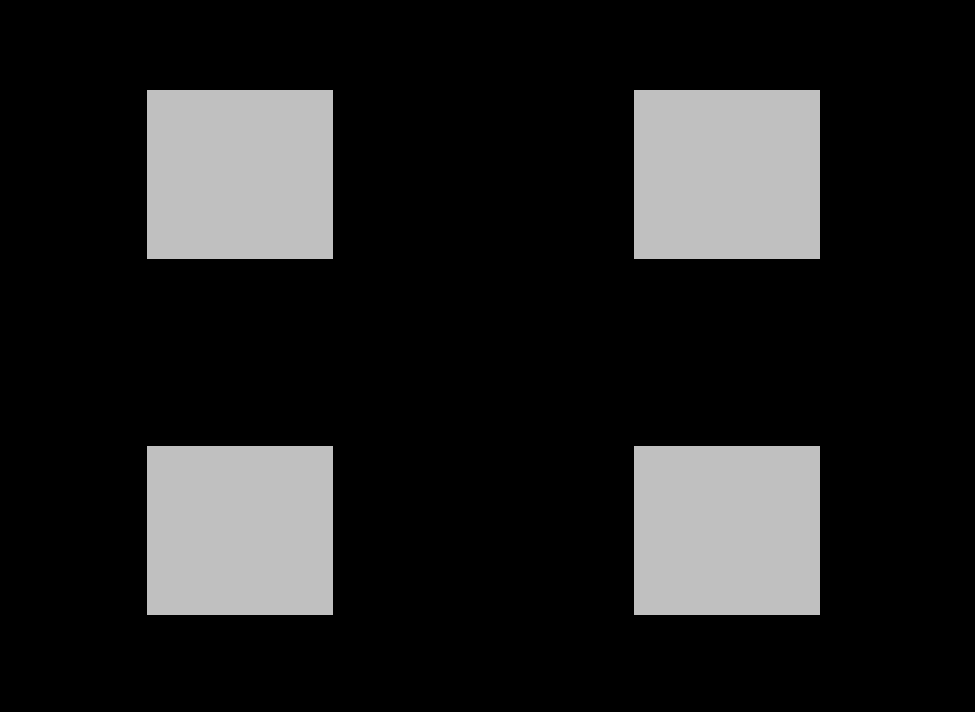
\includegraphics[width=0.8\columnwidth]{figures/B1_ext.png}
			&
			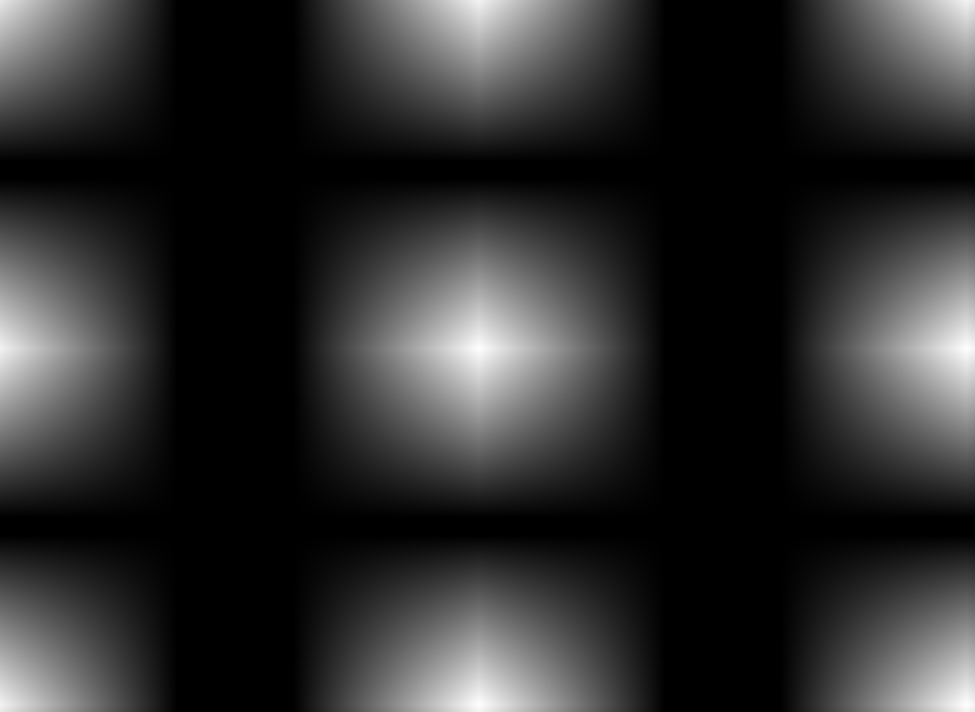
\includegraphics[width=0.8\columnwidth]{figures/B2_ext.png}\\
			B1 & B2\\
			\multicolumn{2}{c}{(quadrupled)}
		\end{tabular}
		\caption{\textit{Above Left:} Image B1 showing a bright square before a darker background. \textit{Above Right:} Result of convolving B1 with itself. B2 was obtained by performing multiplying the Fourier transform of the image with itself in the frequency domain and inverting the result back to the spatial domain. See file \texttt{task\_1d.py} for the code. \textit{Below Left:} Image resulting from quadrupling B1. \textit{Below Right:} Corresponding convolution result.}
		\label{fig:task_1d}
	\end{figure*}
	
	\vspace{12pt}
	\textit{Alternative Explanation:}
	We know what a one-dimensional convolution of a box signal with itself looks like: One box signal is translated in time, such that it appears to be moving over the other. The result of the convolution is basically the changing size of the overlapping area between both signals. In this case, the result is a triangle pulse: While one square is sliding over the other, the overlapping area first increases until both squares overlap completely, after which it decreases again until it becomes zero. A nice animation of this can be found \href{https://en.wikipedia.org/wiki/Convolution#/media/File:Convolution_of_box_signal_with_itself2.gif}{here}.
	
	From that, we can infer what the two-dimensional convolution of the given image, B1, looks like. What was described above basically happens for every row and column of that image. Hence, if we visualized the grayvalue-intensity function in three-dimensional space, the result of this convolution would resemble a cone, if not a pyramid. If we project this intensity function back onto a plane, we obtain the image that results from the convolution. This image would show something like a fading circle, having the highest intensity (brightest color) in its center.
	
	We tried to confirm that our thinking is correct by computing the image actually resulting from the convolution of B1 with itself. To that end, we took advantage of the fact that the convolution in the spatial domain is dual to the multiplication in the frequency domain. The result, which is somewhat different from what we expected, is shown in \Cref{fig:task_1d}. Apparently, this is an unwanted effect of what is called cyclic convolution, which is why that result does not necessarily prove that we are wrong. In fact, it would look a lot like what we imagined if we sliced the image into four pieces and reordered them. To make the test, we performed the convolution on a a slight variation of the previous image, and obtained a resulting image that showed what we were expecting.
	
	\section{Practical Problems}
	
	\subsection{Greyvalue Normalization}
	
	\begin{figure*} [t]
		\centering
		\begin{tabular}{c c}
			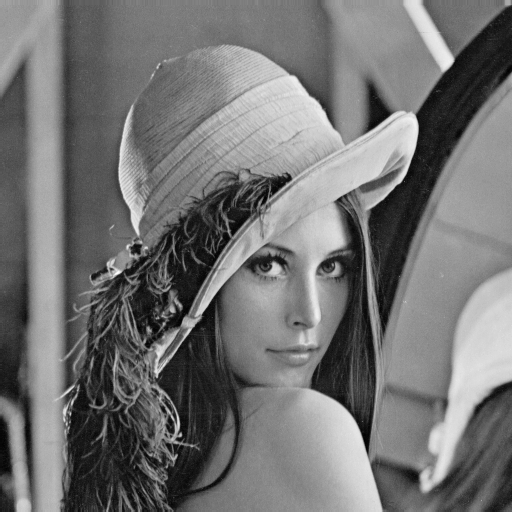
\includegraphics[width=0.8\columnwidth]{figures/original.png}
			&
			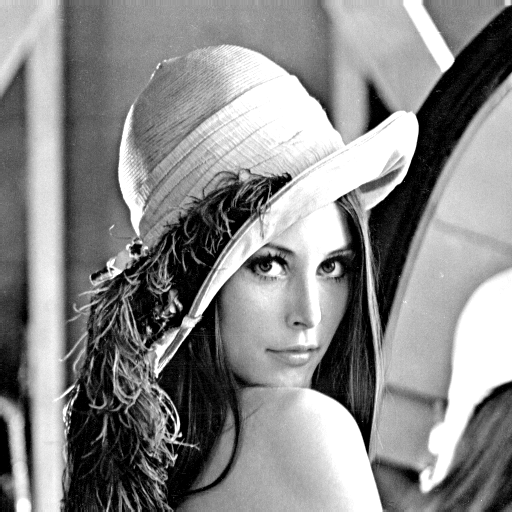
\includegraphics[width=0.8\columnwidth]{figures/normalized.png}
		\end{tabular}
		\caption{\textit{Left:} Original image. \textit{Right:} Image resulting from the \textit{gray-scale normalization}, also referred to as \textit{histogram stretching}. There is a visible enhancement in contrast when compared to the original image.}
		\label{fig:task_2a}
	\end{figure*}
	
	\Cref{fig:task_2a} shows the image obtained after the desired gray-scale normalization was performed. The implementation can be found in \texttt{task\_2a.py}.
	
	\subsection{Fourier-Transform}
	
	The 2D Fourier transform is defined as follows:
	\begin{align*}
	G_{uv} = \frac{1}{M \cdot N} \cdot
	\sum_{m=0}^{M-1} \sum_{n=0}^{N-1} g_{mn} \cdot
	e^{-2 \cdot  \pi \cdot j (\frac{m \cdot u}{M} + \frac{n \cdot v}{N})}
	\end{align*}
	
	It can be shown that this can be broken down into a series of 1D Fourier transforms:
	\begin{align*}
	G_{uv}
	&= \frac{1}{M} \cdot \frac{1}{N} \cdot
	\sum_{m=0}^{M-1} \sum_{n=0}^{N-1} g_{mn} \cdot
	e^{-2 \cdot  \pi \cdot j \frac{m \cdot u}{M}} \cdot
	e^{-2 \cdot  \pi \cdot j \frac{n \cdot v}{N}} \\
	&= \frac{1}{N} \cdot \sum_{n=0}^{N-1}
	e^{-2 \cdot  \pi \cdot j \frac{n \cdot v}{N}} \cdot
	\frac{1}{M} \cdot \sum_{m=0}^{M-1}
	g_{mn} \cdot
	e^{-2 \cdot  \pi \cdot j \frac{m \cdot u}{M}}
	\end{align*}
	
	This shows that, in order to compute a 2D FFT, one can perform 1D FFT on each individual row of the 2D input matrix and then to each of its columns. Of course, this could also be done vice versa: One could first perform it on the columns and then on the rows as well.
	
	Similarly, the 2D inverse Fourier transform can be broken down into a series of 1D inverse Fourier transforms:
	\begin{align*}
	g_{mn}
	&= \sum_{u=0}^{M-1} \sum_{v=0}^{N-1} G_{uv} \cdot
	e^{2 \cdot  \pi \cdot j (\frac{m \cdot u}{M} + \frac{n \cdot v}{N})} \\
	&= \sum_{u=0}^{M-1} \sum_{v=0}^{N-1} G_{uv} \cdot
	e^{2 \cdot  \pi \cdot j \frac{m \cdot u}{M}} \cdot
	e^{2 \cdot  \pi \cdot j \frac{n \cdot v}{N}} \\
	&= \sum_{v=0}^{N-1} e^{2 \cdot \pi \cdot j \frac{n \cdot v}{N}} \cdot
	\sum_{u=0}^{M-1} G_{uv} \cdot
	e^{2 \cdot  \pi \cdot j \frac{m \cdot u}{M}}
	\end{align*}
	
	The same as above holds here as well.
	
	See the file \texttt{task\_2b.py} for the implementation.
	
\end{document}
